\frame
{
\frametitle{\citetitle{MarcoNuno_Revista_2014_10_00}}
\begin{columns}
\column {0.5\textwidth} 
\begin{itemize}
\item La binarización de imágenes es el proceso que convierte el nivel de grises
para distinguir objetos de regiones del fondo.
\item El umbral adaptativo local ofrece una resultados adecuados pero tiene un alto costo computacional. 
\item Se presenta una implementación de hardware reconfigurable para acelerar el algoritmo de Bernsen.
\end{itemize}
 \column {0.5\textwidth} 
    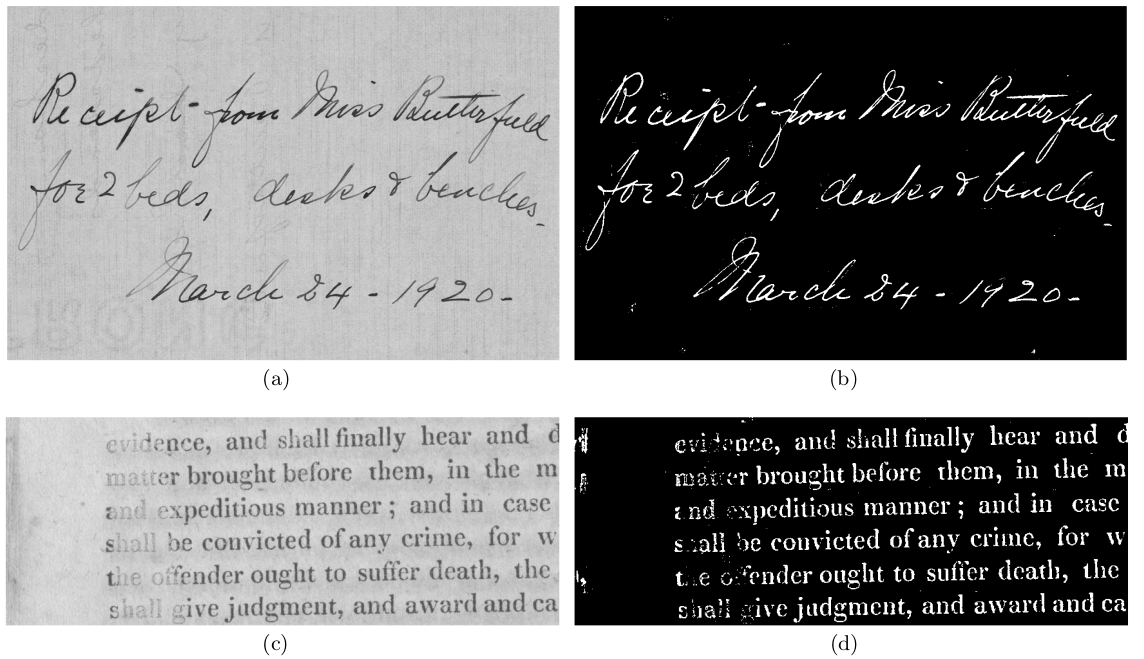
\includegraphics[width=0.9\textwidth]{Figs/2014_Arq_Umbralizacion02}
\end{columns}

\footnotetext[1]{\fullcite{MarcoNuno_Revista_2014_10_00}}
}

\frame
{
\frametitle{Implementación}
\begin{columns}
\column {0.4\textwidth}
\begin{itemize}
\item El algoritmo de Bernsen requiere dos módulos HGW trabajando en paralelo (max y min filtros).
\item Se emplean memorias BlockRAM (embebida dentro del FPGAs). 
\item La unidad de control genera las direcciones de la memoria externa tanto para leer y almacenar los datos de la memoria de entrada y salida, en función del tamaño de la imagen y del núcleo.
\end{itemize}
\column {0.6\textwidth}
\begin{center}
    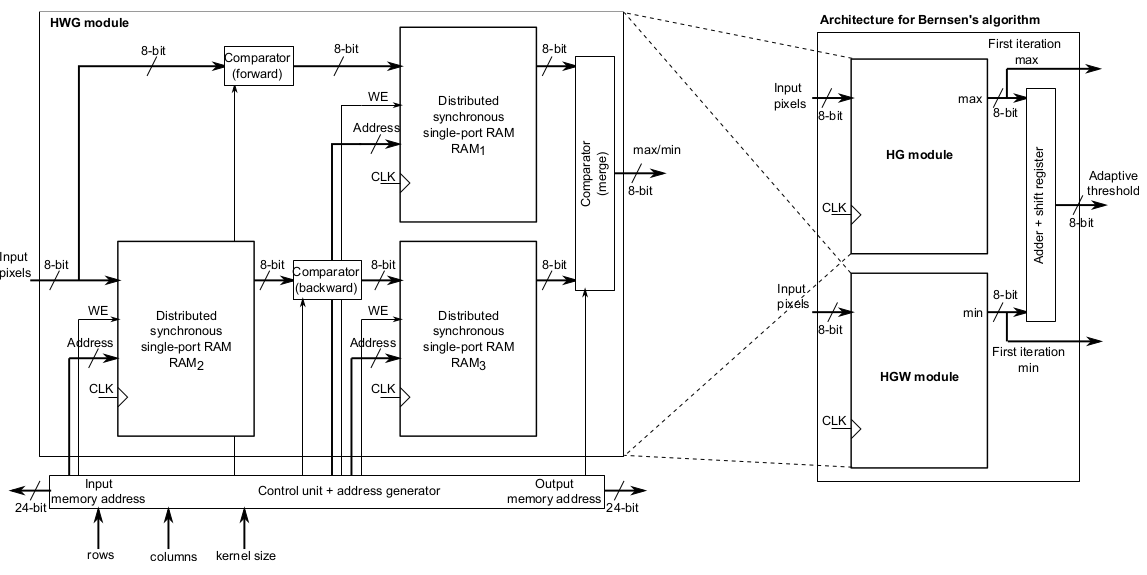
\includegraphics[width=0.99\textwidth]{Figs/2014_Arq_Umbralizacion01}
\end{center}    
\end{columns}
}


\frame
{
\frametitle{Implementación}
\begin{columns}
\column {0.4\textwidth}
Se implemento un Pipeline de 3 etapas:
\begin{itemize}
\item La primera etapa procesa ventanas de tamaño $k$ a partir de los pixeles de entrada. 
\item La segunda etapa comienza a operar después de $k$ ciclos de reloj.
\item La tercera etapa fusiona una vez que la segunda etapa completa el cálculo de $k/2$ muestras de salida.
\end{itemize}

\column {0.6\textwidth}
\begin{center}
    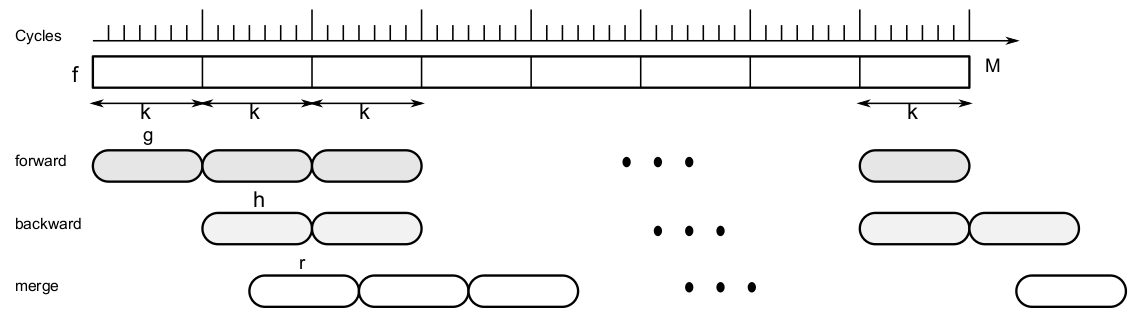
\includegraphics[width=0.99\textwidth]{Figs/2014_Arq_Umbralizacion05}
\end{center}      
\end{columns}

}



\frame
{
\frametitle{Resultados}
\begin{columns}
\column {0.4\textwidth} 
\begin{itemize}
\item FPGAs Atlys y VHDL.

\item Se comparan diferentes tamaños de ventana para una imagen de resolución 2160 $\times$ 1440.
\item Se compararon diferentes tamaños de imagen obteniendo una resolución de video de 30 FPS.
\end{itemize}

 \column {0.3\textwidth} 
    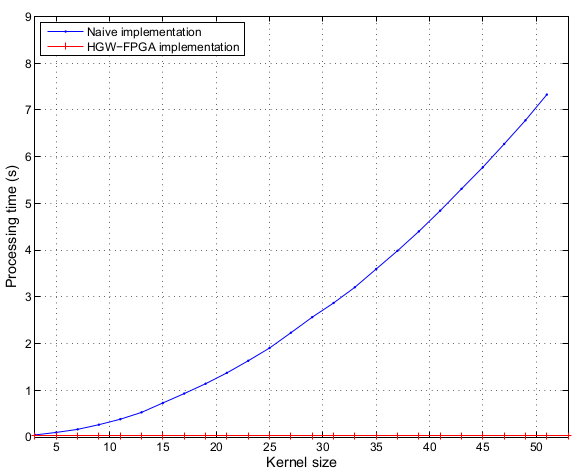
\includegraphics[width=0.9\textwidth]{Figs/2014_Arq_Umbralizacion03}\\
    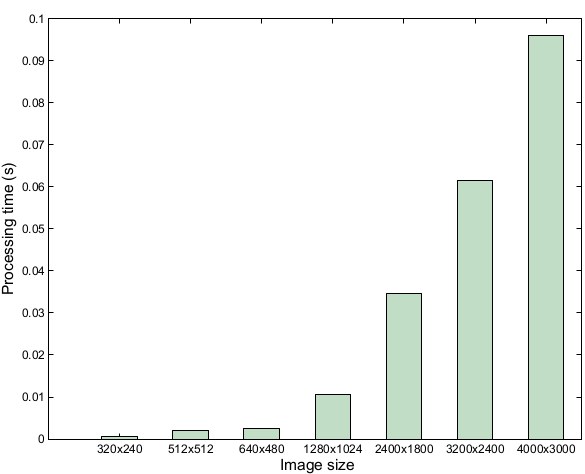
\includegraphics[width=0.9\textwidth]{Figs/2014_Arq_Umbralizacion04}
 \column {0.3\textwidth} 
    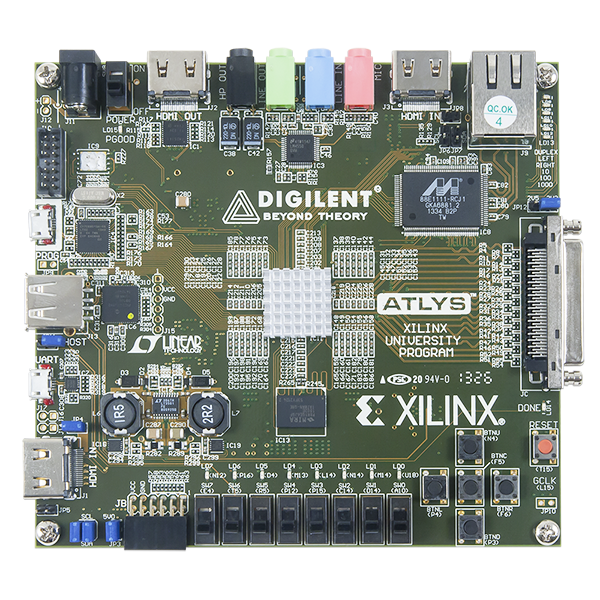
\includegraphics[width=0.9\textwidth]{Figs/atlys-2}\\

\end{columns}

}

